


\begin{frame}{Project C-Manipulator \sof{1}{4}}

%\vspace{1em}

\twocol{0.6}{
\justifying

\vspace{0.75em}
{\bf C-Manipulator}~\cite{Spenneberg2007} is a research project that was 
conducted from 2006 to 2009 at the German Research Center for Artificial 
Intelligence (\lnk{https://robotik.dfki-bremen.de}{DFKI}) in Bremen. 

\vspace{1em}
Its main objective was the development of a {\bf \mbox{manipulator} system for 
deep sea applications} that provides autonomous and assistive functions to the 
system's operators. 

\vspace{1em}
The project used a {\bf hydraulic ORION 7P} by Schilling Robotics as its main 
robotic arm. As main sensors, the system was equipped with two overhead cameras 
used for stereo vision and a single camera mounted to the wrist for visual 
servoing. 

\vspace{1em}
The project was finished successfully with an open water test in coastal 
waters.\vid{publications/2007-01/CManipulator_Open_water_test.mp4}

}{0.3}{
\begin{figure}
\adjincludegraphics[width=0.7\linewidth,valign=t]{cmanipulator/orion7p.jpg}
\vspace{-0.5em}
\caption{\centering \scriptsize The ORION 7P manipulator\protect\linebreak ((c) Schilling Robotics)}
\adjincludegraphics[width=1.\linewidth,valign=b]{cmanipulator/uw-testbed_3D.jpg}
\vspace{-1.5em}
\caption{\centering\scriptsize 3D rendering of the underwater testbed (Jan Albiez, DFKI)}
\end{figure}
}

\vspace{-1em}

\begin{center}
\rule{2cm}{0.4pt}\\[0.5em]
\end{center}

\fc{Spenneberg2007}{publications/2007-01/2007-01}
\end{frame}


\begin{frame}{Project C-Manipulator \sof{2}{4}}

\vspace{1.25em}
\justifying

In~\cite{Hildebrandt2008b} we report on {\bf early results} of the C-Manipulator 
project that introduce a number of improvements over the traditional, manual
control of underwater robotic arms:
\vspace{1em}
\begin{itemize}
	\item We developed a {\bf fast inverse kinematic closed form solution} that 
	allows movements in cartesian space and guarantees numerical stability.
	\item We implemented a two-phase, {\bf semi-autonomous gripping} of 
	objects.\vid{publications/2007-01/CManipulator_Autonomous_underwater_manipulation.mp4}
\end{itemize}

%\vspace{11em}

\twocol{0.23}{
\begin{figure}
\vspace{0.25em}
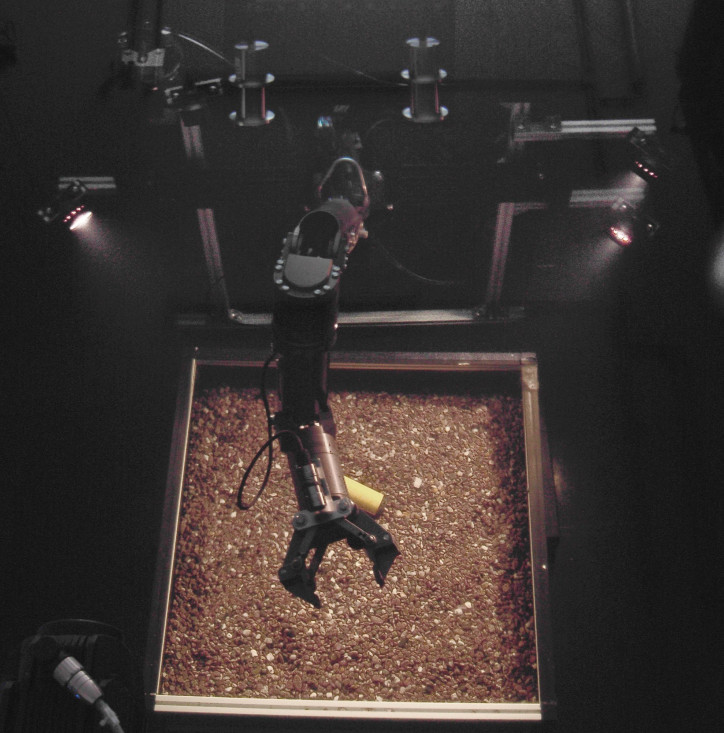
\includegraphics[width=\linewidth]{cmanipulator/in_testbed.jpg}

\vspace{-0.7em}
\caption{\scriptsize The Orion 7P in our underwater 
testbed~\cite{Hildebrandt2008b}.}
\end{figure}
}{0.6}{
\begin{figure}
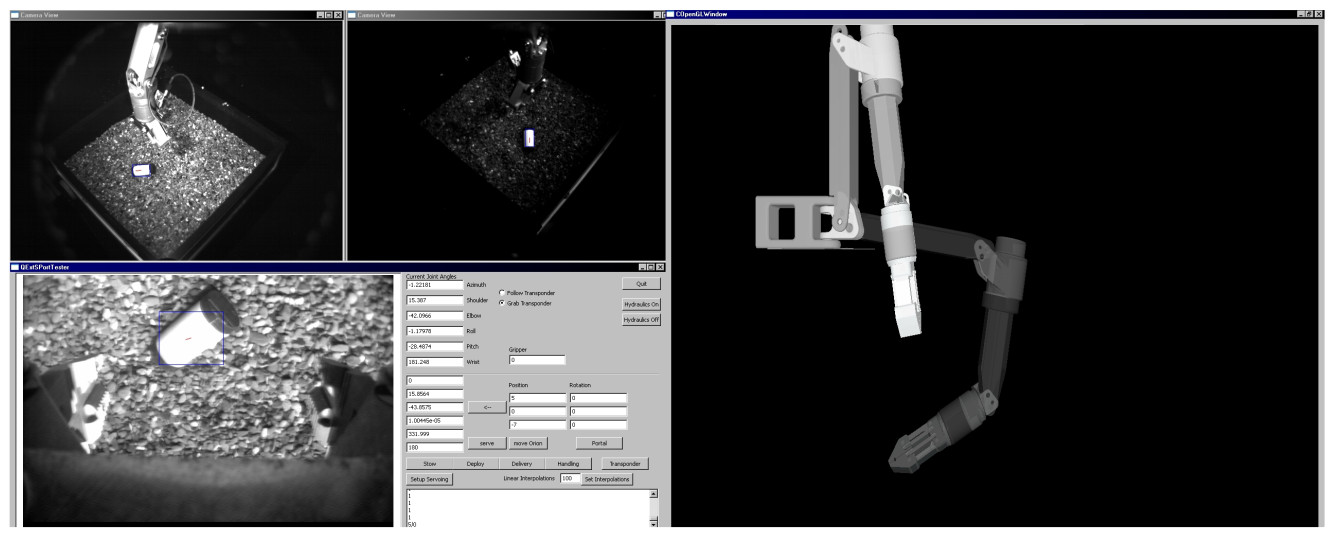
\includegraphics[width=\linewidth]{cmanipulator/control_view.jpg}

\vspace{-0.8em}
\caption{\scriptsize View of the control software. The left side contains all 
three camera images. The right side shows a 3D representation of both the 
current (solid) and future (transparent) positions of the 
manipulator~\cite{Hildebrandt2008b}.}
\end{figure}	
}

%\vspace{-1em}

\begin{center}
\rule{2cm}{0.4pt}\\[0.5em]
\end{center}

\fc{Hildebrandt2008b}{publications/2008-01/2008-01}
\end{frame}

\begin{frame}{Project C-Manipulator \sof{3}{4}}


\twocol{0.25}{
\vspace{-1.5em}
\begin{figure}
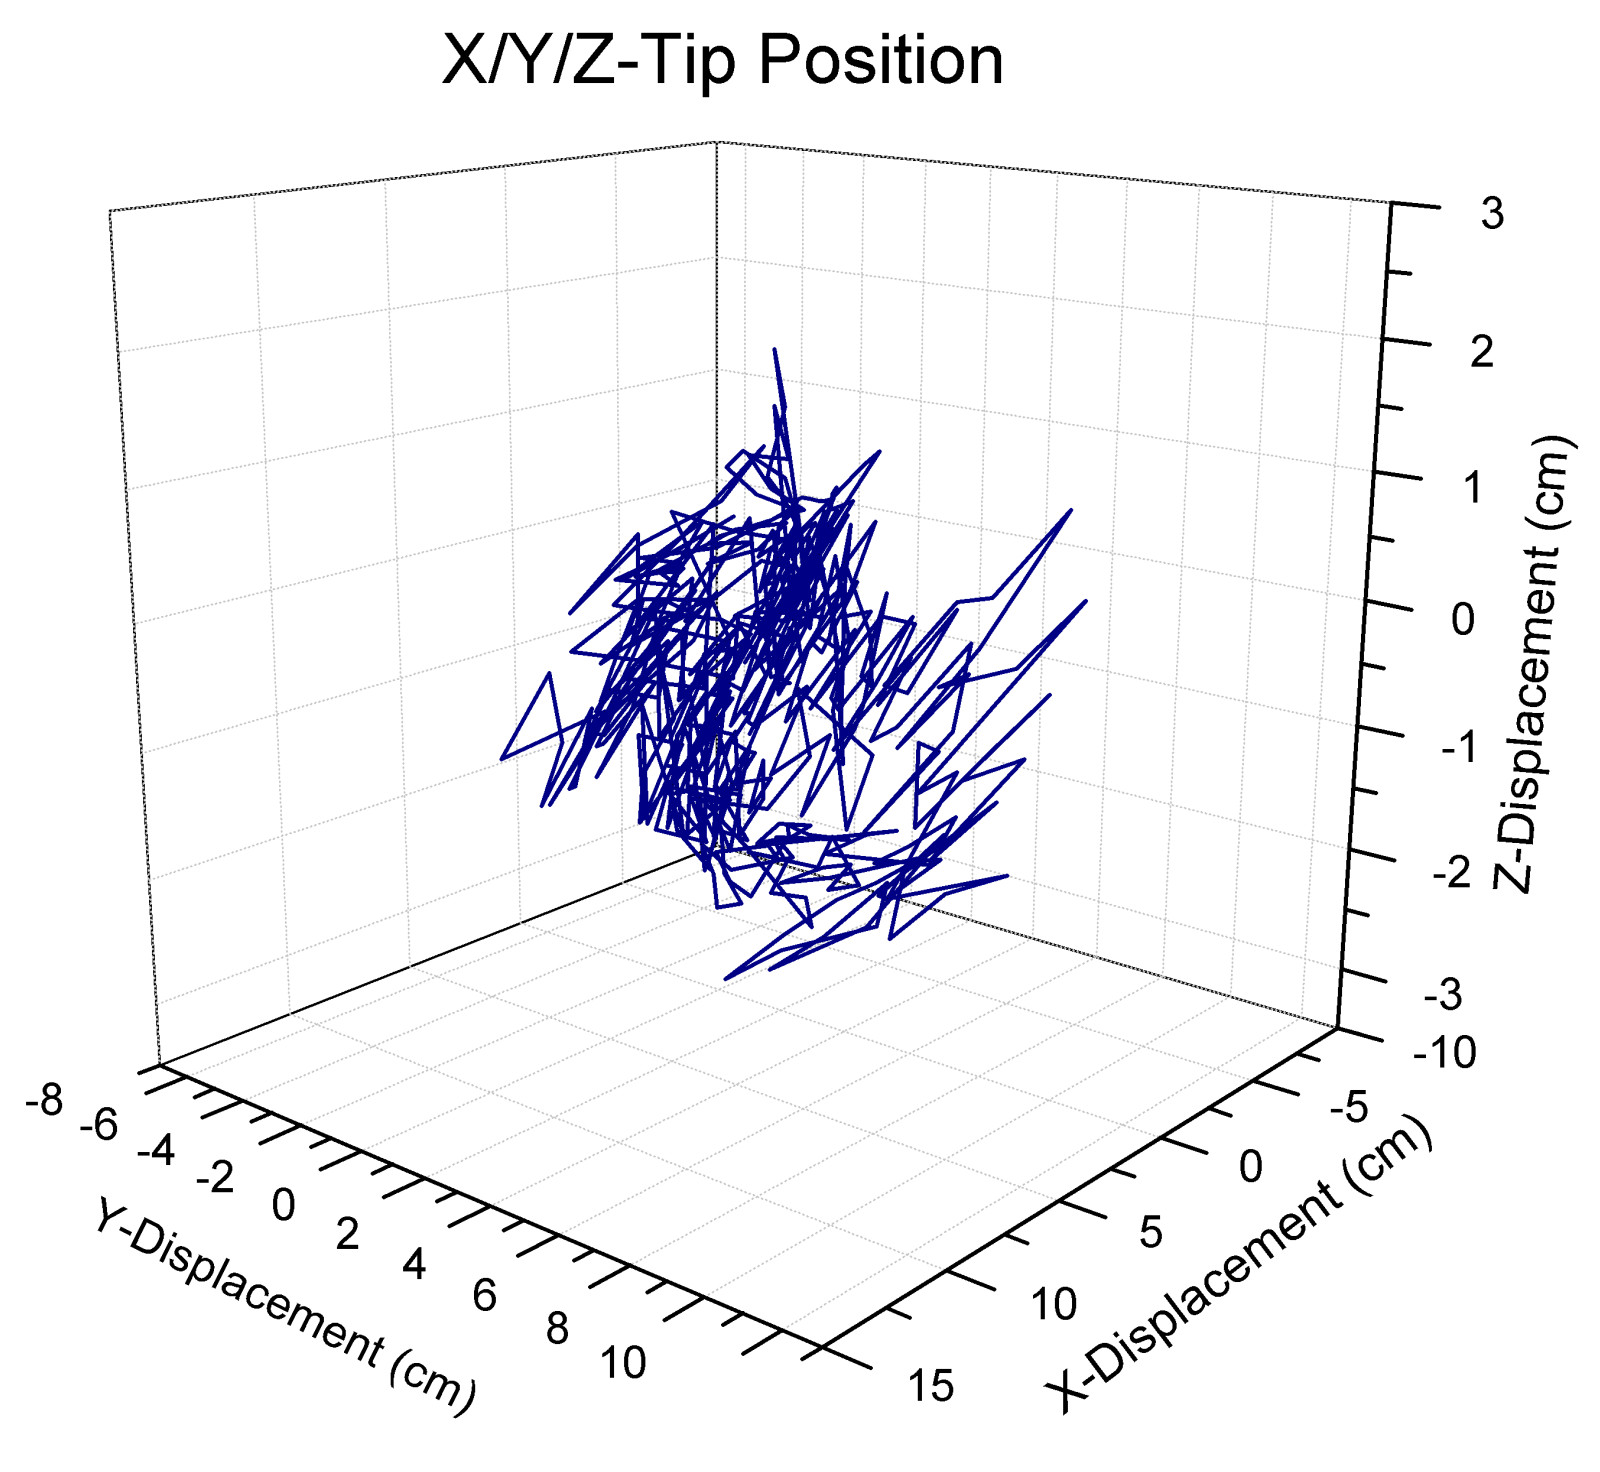
\includegraphics[width=\linewidth]{cmanipulator/motion_comp.jpg}

\vspace{-0.5em}
\caption{\scriptsize 3d plot of tip displacement during movement compensation~\cite{Hildebrandt2009b}.}
\end{figure}

}{0.7}{
\justifying

\vspace{0.5em}
Deep sea robotic arms are usually mounted to remotely operated vehicles (ROV). 
We developed a {\bf novel algorithm to compensate for disturbances} that does 
not rely on the station-keeping algorithm of the ROV but compensates vehicle 
movements directly {\bf via a movement overlay} in the robotic 
arm~\cite{Hildebrandt2009b}.\vid{publications/2009-01/CManipulator_motion_comp.mp4}

}
\vspace{0.5em}

\twocol{0.6}{
\justifying

We {\bf augmented the built-in controller} of the ORION~7P with
a multi-layered controller enabling {\bf high precision end-effector control} 
well beyond the manipulator's original capabilities~\cite{Hildebrandt2009a}. 
We showcased the achievable precision by the automated plugging of an underwater 
connector.\vid{publications/2007-01/CManipulator_GISMA_plug_static.mp4}
}{0.35}{
\vspace{-0.8em}
\begin{figure}
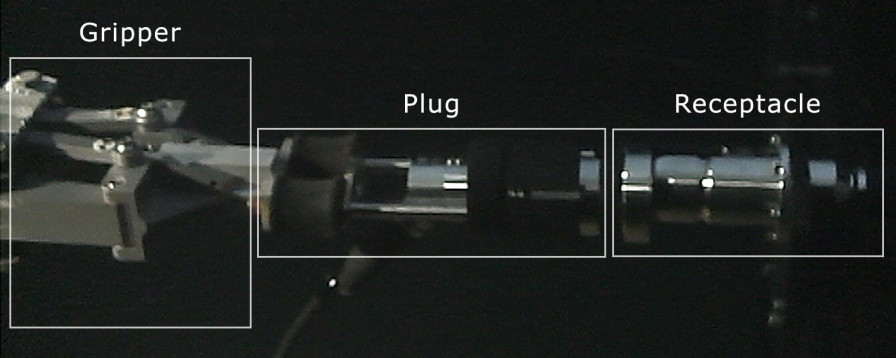
\includegraphics[width=\linewidth]{cmanipulator/precision.jpg}

\vspace{-0.5em}
\caption{\scriptsize Automated plugging of a Gisma Series 80 underwater 
connector~\cite{Hildebrandt2009a}.}
\end{figure}
}

\begin{center}
\rule{2cm}{0.4pt}\\[0.5em]
\end{center}

\fc{Hildebrandt2009b}{publications/2009-01/2009-01}\\[1em]
\fc{Hildebrandt2009a}{publications/2009-02/2009-02}
\end{frame}



\begin{frame}{Project C-Manipulator \sof{4}{4}}

%\vspace{1em}
%\justifying

\twocol{0.6}{
\justifying

\vspace{1em}
One of the primary tasks of modern ROV deployment is {\bf intervention work}. 
Intervention in these cases consists of tasks like opening fixtures, or plugging
connections.

\vspace{1em}
Robotic operators have to rely solely on visual feedback and their experience
to determine if in a given situation a desired position is reachable, and how 
much dexterity will be available to perform the intended task.

\vspace{1em}
We introduced a {\bf methodology to represent workspace properties} like 
remaining dexterity with {\bf respect to tele-operation tasks}~\cite{Albiez2009}.
The information gained can be used as a signal to an operator or as the basis 
for motion commands to the ROV carrying the robot arm.

}{0.3}{
\begin{figure}
\adjincludegraphics[width=0.9\linewidth,valign=t]{cmanipulator/workspace.jpg}
\vspace{-0.5em}
\caption{\scriptsize Nominal workspace of the ORION 7P~\cite{Albiez2009}. }
\adjincludegraphics[width=0.9\linewidth,valign=b]{cmanipulator/dexterous.jpg}
\vspace{-0.5em}
\caption{\scriptsize Dexterous workspace of the ORION 7P for a 
front-down position of the gripper~\cite{Albiez2009}.}
\end{figure}
}

\vspace{-0.5em}

\begin{center}
\rule{2cm}{0.4pt}\\[0.5em]
\end{center}

\fc{Albiez2009}{publications/2009-03/2009-03}
\end{frame}

